\section{Predictive control strategy}\label{sec:ch6_MPC}
This section discusses the details on formulating the adaptive predictive control problem based on the \gls{lpv} model~\eqref{eq:ch6_IOmodel} with varying time delay. The reader is referred to~\cite{mpcbook} for basic terminology and details related to \gls{mpc}.

\subsection{Optimization problem formulation}\label{sec:ch6_probform}
The \gls{mpc} problem is formulated based on a performance index which reflects the control objectives and a set of constraints including the equalities due to the \gls{lpv} prediction model~\eqref{eq:ch6_IOmodel}. We consider a quadratic performance index~$J$ that penalizes output tracking error and deviation of inputs from steady-state targets, i.e.,

\small
\vspace{-1em}
\begin{multline*}
    J(k) = \sum\limits_{j=1}^{N_{\text{p}}(k)}\frac{1}{2}\Vert W_y(k+j)\cdot(y(k+j)-y_r(k+j))\Vert_2^2 \\ + \sum\limits_{j=0}^{N_{\text{p}}(k)-1} \frac{1}{2}\Vert W_u(k+j)\cdot (u(k+j)-u_r(k+j))\Vert_2^2
\end{multline*}
\normalsize
where $W_y(k)$ and $W_u(k)$ denote weights on output and input respectively at time step $k$ whereas $y_r$ and $u_r$ denote their target values. The prediction horizon $N_{\text{p}}(k)$ determines the number of decision variables i.e., the inputs and outputs in prediction to be optimized.
Considering simple bounds on the decision variables, the \gls{mpc} problem to be solved at each time step is the constrained optimization problem 

\small
\vspace{-1em}
\begin{subequations}\label{eq:ch6_mpcopt}
\begin{align}
  & \min_{u(\cdot), y(\cdot)} J(k) \nonumber\\
  \text{s.t.}\quad y(k+l) &= \sum_{j=1}^{n_x} A_j(p) y(k+l-j) %\notag\\ &\quad 
  + \sum_{j=1}^{n_x+n_d(k)+1} B_j(p) u(k+l-j)\notag\\
   &= M(p, n_d(k))  \cdot\phi(k+l-1),\forall l \in \{1,\ldots,N_{\text{p}}\} \label{eq:ch6_predmodeleqs}\\
  u(k+j) &= u(k+N_{\text{u}}-1), \forall j \in \{N_{\text{u}},\ldots,N_{\text{p}}\}\label{eq:ch6_ctrlhor}\\  
  y(k) &= y_0 \label{eq:ch6_inity}\\
  \phi(k) &= \phi_0~\label{eq:ch6_initphi}\\
  y_{\text{l}}(k+j) & \leq y(k+j) \leq y_{\text{u}}(k+j), \forall j \in \{1,\ldots,N_{\text{p}}\}\label{eq:ch6_ybounds}\\
  u_{\text{l}}(k+j) & \leq u(k+j) \leq u_{\text{u}}(k+j), \forall j \in \{1,\ldots,N_{\text{u}}\} \label{eq:ch6_ubounds}
\end{align}
\end{subequations}
\normalsize
where $M$ in~\eqref{eq:ch6_predmodeleqs} is the matrix of parameter-dependent model coefficients such that $\phi(k) = [y^{\top}(k),y^{\top}(k-1),\ldots,y^{\top}(k-n_x), u^{\top}(k-1), u^{\top}(k-2),\ldots,u^{\top}(k-n_x-n_d(k)-1)]^{\top}$. The upper and lower bounds on any variable $z$ are denoted as $z_{\text{u}}$ and $z_{\text{l}}$, respectively. The initial condition \eqref{eq:ch6_inity}-\eqref{eq:ch6_initphi} in the \gls{io} case is provided via the measured output feedback $y_0$, and vector $\phi_0$ which also includes the known past sequence of inputs and outputs. The input sequence that is optimized is typically restricted to fewer variables for trading-off control performance with computations via the control horizon~($N_{\text{u}}$) constraint~\eqref{eq:ch6_ctrlhor}, i.e., by tuning the parameter~$N_{\text{u}}$ such that $1\leq N_{\text{u}}<N_{\text{p}}$, where $N_{\text{p}}>n_d$. 
Note that the future values of parameters~$p$ can be incorporated as they may be known and in that case~$p$ represents~$p(k+l)$ in the \gls{lpv} model~\eqref{eq:ch6_predmodeleqs}.

\subsection{Adaptation with workload variations}
\label{sec:ch6_cases}
In \gls{ibc}, besides control computation and actuation time, the sensor-to-actuator delay mainly includes the sensing time. We assume that the delay due to control computation and actuation are fixed, but the sensing delay may vary as explained in Section~\ref{sec:ch6_IBCworkvar}. 
We propose to adapt the controller at runtime to make immediate use of the latest available measurement in order to maximize \gls{qoc}. The basic idea is to have the time delay as a variable parameter based on which the model is adapted as explained in Section~\ref{sec:ch6_adaptmodel}. The varying parameter ($n_d$) is then kept constant in prediction as shown in~\eqref{eq:ch6_predmodeleqs}. Since the actuation rate can be constant thanks to pipelining, a new control action is computed at each time step with a \gls{zoh} during the sampling period. 

\begin{figure}[t]
\centerline{
    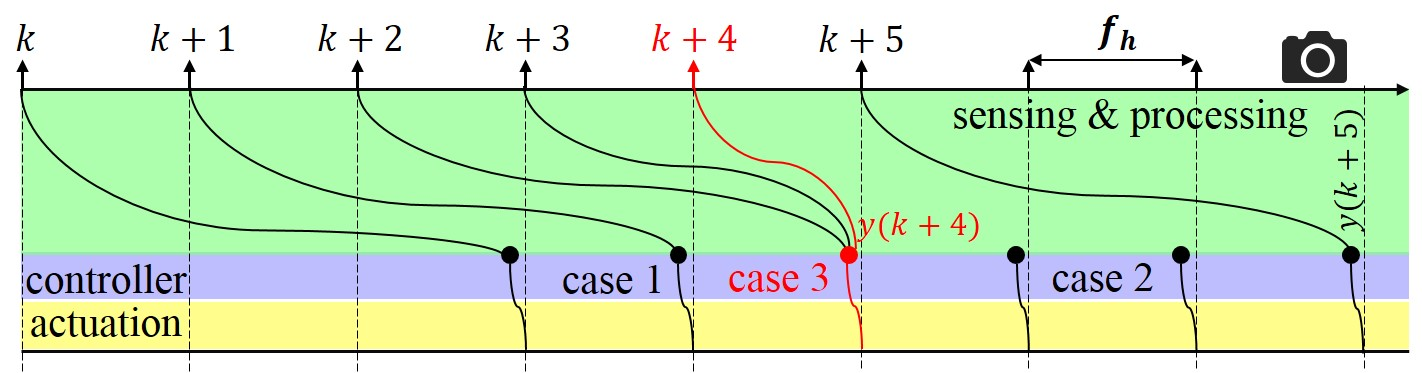
\includegraphics[width=0.9\textwidth]{images/pIBCv.jpg}
    }
    %\vspace{-1em}
    \caption{Illustration of cases described in Section~\ref{sec:ch6_cases}.
    The samples $k+3$ and $k+4$ have lower workloads and thus the latest output measurement $y(k+4)$ is available within one $\fh$. Note that for case 2, the latest measurements are not available and thus $u(k+i)$ is computed based on the \gls{mpc} prediction model.}
    \label{fig:ch6_pIBCvariations}
    \vspace{-2em}
\end{figure}
The following three cases may occur at each time step due to varying sensing delay (illustrated in Fig.~\ref{fig:ch6_pIBCvariations}): 
\begin{enumerate}
\item 
the new measurement is available with the same sensing delay as in the previous step: in this case the parameter $n_d$ is kept constant and the initial condition for computing the new control input is updated as usual, i.e., $\phi=[y^{\top}(k-1),\ldots,y^{\top}(k-n_x),\cdots]^{\top}$ becomes $\phi=[y(k),\ldots,y^{\top}(k-n_x+1),\cdots]^{\top}$; 
\item the sensing delay is increased compared to the previous step as the latest measurement is not available: in this case, the prediction is done starting from the old measurement, i.e., the delay parameter $n_d$ is incremented by 1 and the stack of past outputs in $\phi$ is not updated. 
\item the sensing delay is reduced by one or more steps: when multiple pipes finish processing a corresponding sequence of frames, both the latest measurement(s) along with the past measurements now available are fed to the controller and $n_d$ is accordingly reduced where, from an implementation perspective, the output stack in the initial condition $\phi$ is updated as in case 1 discussed above and the same procedure is then repeated as many times as the reduction in $n_d$ before computing the next control input.
\end{enumerate} 

Since a new control input is applied at each step, the stack of past inputs in the initial condition vector~$\phi$ is always updated by a unit shift in all the three cases, i.e., in $\phi=[\cdots, u^{\top}(k-1),\ldots,u^{\top}(k-n)]^{\top}$ becomes $\phi = [\cdots, u^{\top}(k),\ldots,u^{\top}(k-n+1)]^{\top}$. In conclusion, until the next measurement is available, the proposed controller compensates for the delay by making use of the prediction model to implicitly estimate the current status of the system (without a  separate open-loop estimator) while accordingly computing an optimal action that satisfies given constraints. 

The ordering of measurements is important in the current \gls{mpc} implementation since we do not want to allow discarding measurements (as the application we consider, in Section~\ref{sec:lkas_case_Study}, is safety-critical). 
This can be considered as a limitation of the current approach. Ordering means that the latest measurement $y(k+i)$ is updated in the output stack $\phi$ iff the previous measurements $y(k+j),\ j<i,$ were already updated in $\phi$.